\subsubsection*{Problem Statement Question 3}
A cylindrical limb segment in a musculoskeletal model has a radius of \textbf{5.5 units} and a height of \textbf{9.5 units}. The \textbf{tendon stress density} at a point $(x,y,z)$ within the segment is defined by:
\[ P(x, y, z) = 354.62x^2 + 354.62y^2 \]
Compute the total tendon stress in the segment using \textbf{cylindrical coordinates}.

\subsubsection*{Solution}
The total tendon stress $S$ is defined as the triple integral of the density function $P(x, y, z)$ over the cylindrical region:
\[ S = \iiint_V P(x, y, z) \, dV \]

Converting the density function into cylindrical coordinates ($x^2 + y^2 = r^2$):
\[ P(r, \theta, z) = 354.62r^2 \]

The volume element in cylindrical coordinates is $dV = r \, dr \, d\theta \, dz$. The limits of integration for the cylinder are:
\[ 0 \le r \le 5.5, \quad 0 \le \theta \le 2\pi, \quad 0 \le z \le 9.5 \]

Applying the iterated integration process step-by-step:
\[ S = \int_{0}^{9.5} \int_{0}^{2\pi} \int_{0}^{5.5} 354.62r^3 \, dr \, d\theta \, dz \]

\vspace{1cm}
\noindent\textbf{Step 1: Integrate with respect to $r$.}

\[ \int_{0}^{5.5} 354.62r^3 \, dr = 354.62 \left[ \frac{r^4}{4} \right]_{0}^{5.5} \]
\[ = 354.62 \left( \frac{14641}{64} \right) = 81124.8759 \]
\[ \Rightarrow S = \int_{0}^{9.5} \int_{0}^{2\pi} 81124.8759 \, d\theta \, dz \]

\vspace{1cm}
\noindent\textbf{Step 2: Integrate with respect to $\theta$.}

\[ \int_{0}^{2\pi} 81124.8759 \, d\theta = 81124.8759 \Big[\theta\Big]_{0}^{2\pi} = 162249.7518\pi \]
The integral expression simplifies to:
\[ S = \int_{0}^{9.5} 162249.7518\pi \, dz \]

\vspace{1cm}
\noindent\textbf{Step 3: Integrate with respect to $z$.}

\[ \int_{0}^{9.5} 162249.7518\pi \, dz = 162249.7518\pi [z]_{0}^{9.5} = 162249.7518\pi (9.5) \]

\vspace{1cm}
\noindent\textbf{Step 4: Simplify the result.}

\[ S = 1540798.1171\pi \approx \boxed{4,842,364.3742} \]

Thus, the total tendon stress distributed in the segment is exactly $\mathbf{4,842,364.3742}$.

\subsubsection*{MATLAB Verification \& Conclusion}
\textbf{MATLAB Code:}
\begin{mdframed}[backgroundcolor=gray!10]
	\inputminted{matlab}{codes/q3s4.m}
\end{mdframed}

\vspace{1cm}
\noindent\textbf{MATLAB Screenshot:}
\begin{figure}[H]
	\begin{center}
		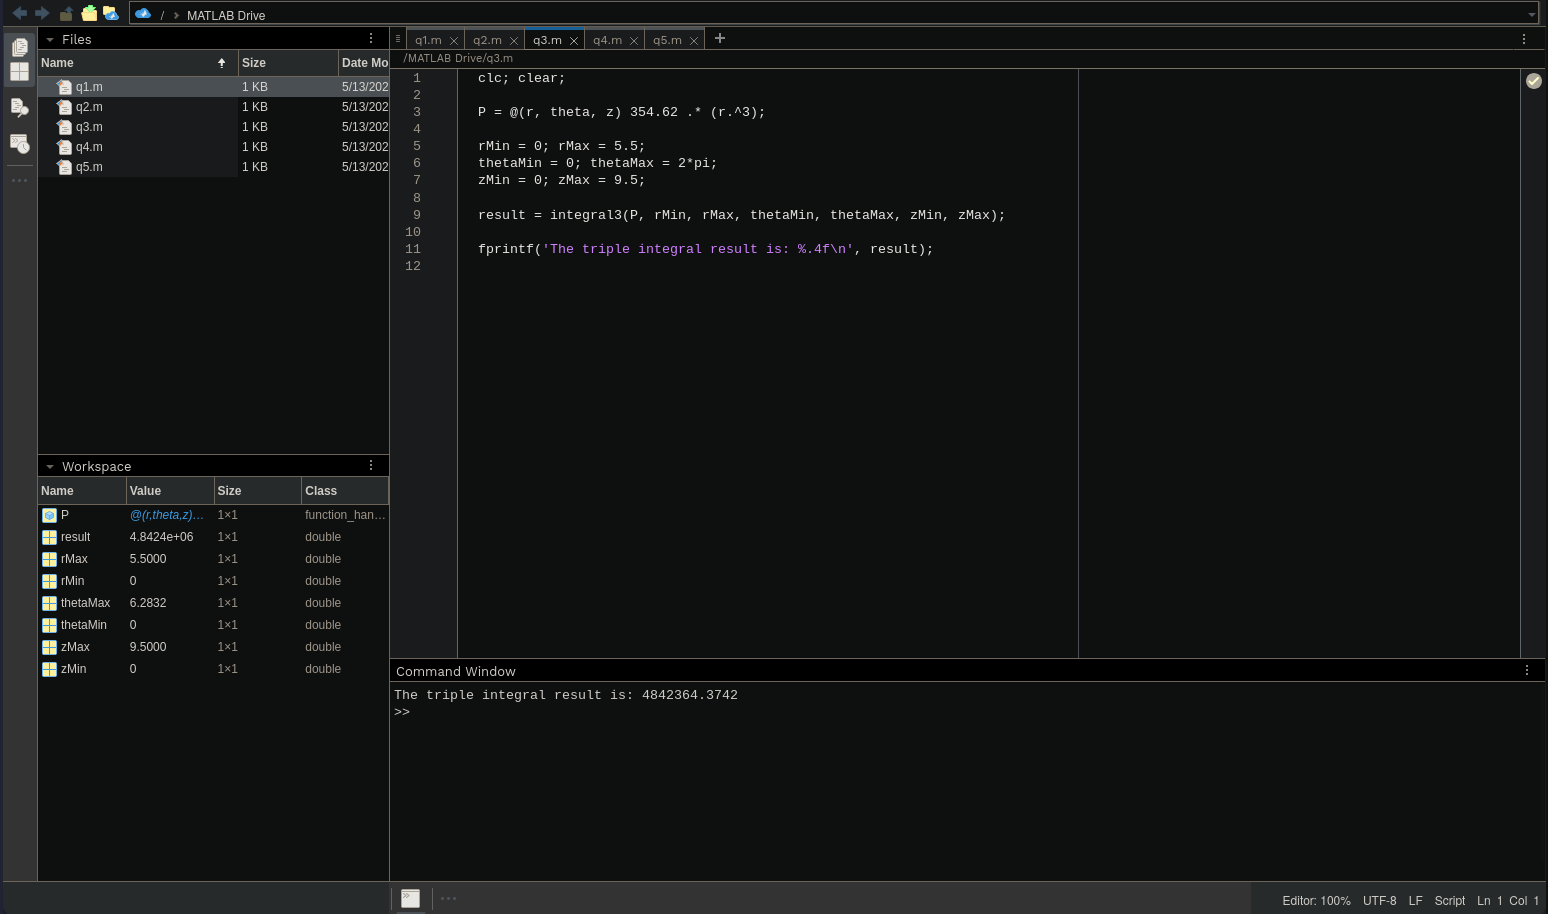
\includegraphics[width=0.95\textwidth]{figures/stu4q3.png}
	\end{center}
\end{figure}

\vspace{1cm}
\noindent\textbf{Conclusion:}

The total tendon stress calculated by using cylindrical coordinates gives the \textbf{same} result as the MATLAB script.
